\begin{figure}
  \caption{topology results for \gottardo}
  \label{pgfplot:20130905}
  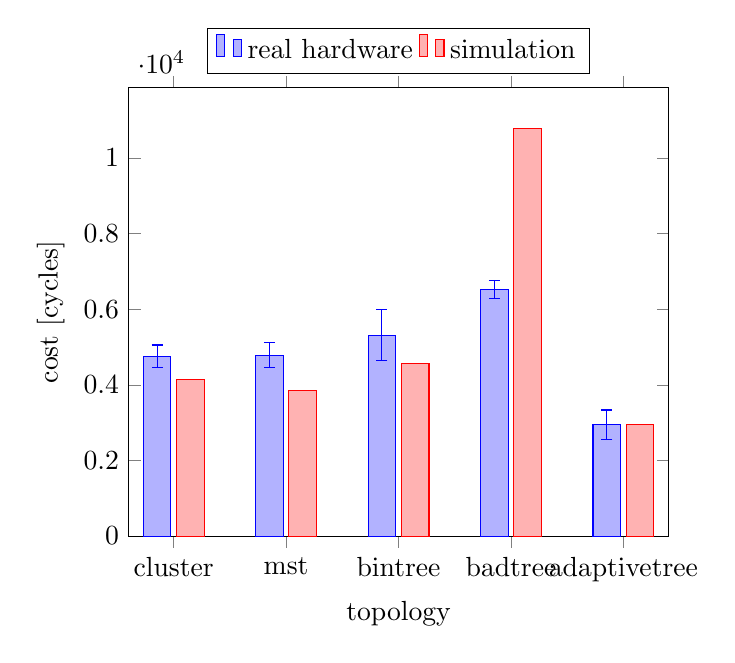
\begin{tikzpicture}[scale=1]
    \begin{axis}[ybar,ymin=0,symbolic x coords={cluster,mst,bintree,badtree,adaptivetree},xtick=data,error bars/y dir=both,error bars/y explicit,legend style={ at={(0.5,1.03)}, anchor=south },legend columns=2,xlabel={topology},ylabel={cost [cycles]}]
      \addplot coordinates {
        (cluster,     4757.069778) +- (295.052921,295.052921)
        (mst,         4782.338222) +- (334.200860,334.200860)
        (bintree,     5311.554222) +- (672.510361,672.510361)
        (badtree,     6527.362667) +- (240.869460,240.869460)
        (adaptivetree,2947.144889) +- (386.628248,386.628248)
      };
      \addplot coordinates {
        (cluster,     4136.839016)
        (mst,         3843.087380)
        (bintree,     4564.574037)
        (badtree,     10779.869076)
        (adaptivetree,2947.144889)
      };
      \legend{real hardware, simulation};
    \end{axis}
  \end{tikzpicture}
\end{figure}
